\documentclass[
	fontsize=10pt, % Base font size
	twoside=false, % Use different layouts for even and odd pages (in particular, if twoside=true, the margin column will be always on the outside)
	%open=any, % If twoside=true, uncomment this to force new chapters to start on any page, not only on right (odd) pages
	%chapterprefix=true, % Uncomment to use the word "Chapter" before chapter numbers everywhere they appear
	%chapterentrydots=true, % Uncomment to output dots from the chapter name to the page number in the table of contents
	numbers=noenddot, % Comment to output dots after chapter numbers; the most common values for this option are: enddot, noenddot and auto (see the KOMAScript documentation for an in-depth explanation)
	%draft=true, % If uncommented, rulers will be added in the header and footer
	%overfullrule=true, % If uncommented, overly long lines will be marked by a black box; useful for correcting spacing problems
]{kaohandt}

% Choose the language
\usepackage[english]{babel} % Load characters and hyphenation
\usepackage[english=british]{csquotes}	% English quotes

% Load the bibliography package
\usepackage{kaobiblio}
\addbibresource{main.bib} % Bibliography file

% Load mathematical packages for theorems and related environments
\usepackage{kaotheorems}

% Load the package for hyperreferences
\usepackage{kaorefs}

% Set the paths where to look for images
\usepackage{subcaption}
\graphicspath{{examples/report/img/}{img/}}

\begin{document}

\title{Operation T-REx}
\author[FM]{Federico Marotta}
\date{December 2019}
\maketitle

\section{Introduction}
\labsec{intro}

Ever since the sequence of the human genome was made available some 20 
years ago, \sidecite[-1\baselineskip]{Lander2001a} one of the most 
compelling goals in both science and medicine has been that of finding 
the genetic variants associated to diseases.

% The first attempts relied on statistical association tests, like the 
% $\chi^2$ test, to identify the genetic variants that are more likely to 
% occur in ill rather than healthy individuals. \sidecite{Visscher2012a} 
% Despite its successes, the power of this approach is hampered by the 
% fact that there are so many genetic variants (on average, the DNA 
% sequences of two non-related people differ of about one letter every one 
% thousand \sidecite{Durbin2010}), most of which, the so-called rare 
% variants, appear only in a tiny fraction of individuals.

In 2015 it was proposed a new method, 
\sidecite[-1.1cm]{Gamazon2015a} dubbed Transcriptome-Wide 
Association Study (TWAS), which consists of using the genetic variants 
to predict gene expression, and then finding associations between the 
predicted expression and a disease. The first advantage is that it is 
possible to avoid a direct measurement of gene expression, which can be 
expensive or even impossible for certain tissues. But another, more 
subtle advantage is that predicted values are less noisy than the real 
ones, because they do not include the environmental component of 
expression (\refeq{expr}). In view of this method, predicting gene 
expression is a relevant problem.

A gene is a region of DNA, and its expression can be defined as the 
amount of RNA molecules that originate from that region 
(\vreffig{response}). This amount is different in different individuals, 
and our goal is to predict these differences.

\begin{marginfigure}[-3.8cm]
  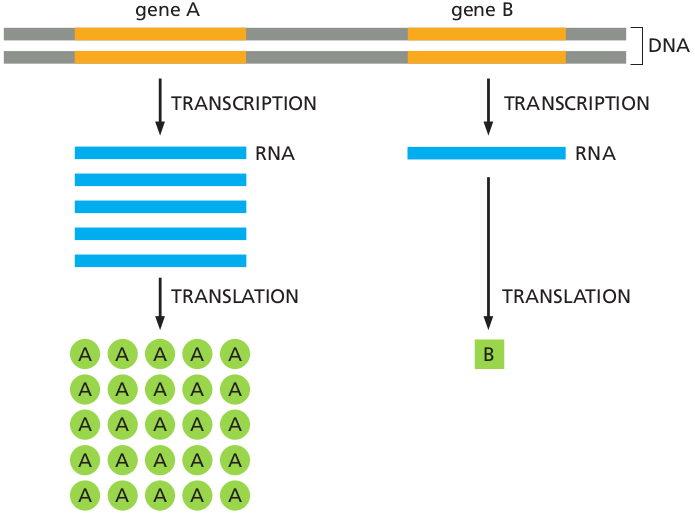
\includegraphics{response}
  \caption{Each gene is \enquote{transcribed} into many RNA molecules, 
which then are \enquote{translated} into proteins.}
  \labfig{response}
\end{marginfigure}

As regards the DNA itself, in this context it can be regarded as a 
3-billion letter long string, different for each individual. Most of the 
positions in the sequence are the same, but there are some specific
positions, called polymorphic loci, which harbour different letters in 
different people (\reffig{predictorsA}). There are many kinds of 
differences, but, as similar works do, 
\sidecite[-8.6cm]{Nagpal2019} here we will focus only on 
single-letter differences such that in the population only two letters 
are present, \ie we will only consider those positions that can be in 
two states.

\begin{marginfigure}[-1.5cm]
\setlength{\tabcolsep}{2pt}
\scalebox{0.7}{%
\begin{subfigure}{\textwidth}
  \caption{}
  \labfig{predictorsA}
  \small
  \texttt{%
  \begin{tabular}{l c c c c c c c c c c c c c c c c c c}
	\textsf{Alice\hspace{.2cm}} & A & T & G & \cellcolor{yellow}G	& T & G & \cellcolor{cyan}C		& T & G & T & C & T & C & C & T & G & \cellcolor{red}T	& C \\
	\textsf{Bob\hspace{.2cm}}   & A & T & G & \cellcolor{yellow}G	& T & G & \cellcolor{cyan}C		& T & G & T & C & T & C & C & T & G & \cellcolor{cyan}C	& C \\
	\textsf{Craig\hspace{.2cm}} & A & T & G & \cellcolor{green}A	& T & G & \cellcolor{green}A	& T & G & T & C & T & C & C & T & G & \cellcolor{cyan}C	& C \\
	\textsf{Dave\hspace{.2cm}}  & A & T & G & \cellcolor{green}A	& T & G & \cellcolor{cyan}C		& T & G & T & C & T & C & C & T & G & \cellcolor{cyan}C	& C \\
	\textsf{Eve\hspace{.2cm}}   & A & T & G & \cellcolor{yellow}G	& T & G & \cellcolor{green}A	& T & G & T & C & T & C & C & T & G & \cellcolor{red}T	& C \\
	\textsf{Frank\hspace{.2cm}} & A & T & G & \cellcolor{yellow}G	& T & G & \cellcolor{green}A	& T & G & T & C & T & C & C & T & G & \cellcolor{cyan}C	& C \\
  \end{tabular}}
\end{subfigure}
}

\scalebox{0.7}{%
\begin{subfigure}{\textwidth}
  \caption{}
  \labfig{predictorsB}
  \small
  \texttt{%
  \begin{tabular}{l c c c c c c c c c c c c c c c c c c}
	\textsf{Alice\hspace{.2cm}} & \phantom{A} & \phantom{A} & \phantom{A} & 0 & \phantom{A} & \phantom{A} & 0 & \phantom{A} & \phantom{A} & \phantom{A} & \phantom{A} & \phantom{A} & \phantom{A} & \phantom{A} & \phantom{A} & \phantom{A} & 1 & \phantom{A} \\
	\textsf{Bob\hspace{.2cm}}   & \phantom{A} & \phantom{A} & \phantom{A} & 0 & \phantom{A} & \phantom{A} & 0 & \phantom{A} & \phantom{A} & \phantom{A} & \phantom{A} & \phantom{A} & \phantom{A} & \phantom{A} & \phantom{A} & \phantom{A} & 0 & \phantom{A} \\
	\textsf{Craig\hspace{.2cm}} & \phantom{A} & \phantom{A} & \phantom{A} & 1 & \phantom{A} & \phantom{A} & 1 & \phantom{A} & \phantom{A} & \phantom{A} & \phantom{A} & \phantom{A} & \phantom{A} & \phantom{A} & \phantom{A} & \phantom{A} & 0 & \phantom{A} \\
	\textsf{Dave\hspace{.2cm}}  & \phantom{A} & \phantom{A} & \phantom{A} & 1 & \phantom{A} & \phantom{A} & 0 & \phantom{A} & \phantom{A} & \phantom{A} & \phantom{A} & \phantom{A} & \phantom{A} & \phantom{A} & \phantom{A} & \phantom{A} & 0 & \phantom{A} \\
	\textsf{Eve\hspace{.2cm}}   & \phantom{A} & \phantom{A} & \phantom{A} & 0 & \phantom{A} & \phantom{A} & 1 & \phantom{A} & \phantom{A} & \phantom{A} & \phantom{A} & \phantom{A} & \phantom{A} & \phantom{A} & \phantom{A} & \phantom{A} & 1 & \phantom{A} \\
	\textsf{Frank\hspace{.2cm}} & \phantom{A} & \phantom{A} & \phantom{A} & 0 & \phantom{A} & \phantom{A} & 1 & \phantom{A} & \phantom{A} & \phantom{A} & \phantom{A} & \phantom{A} & \phantom{A} & \phantom{A} & \phantom{A} & \phantom{A} & 0 & \phantom{A} \\
  \end{tabular}}
\end{subfigure}
}
\caption{(a) Examples of DNA sequences; polymorphic loci are highlighted
with different colours. (b) Predictors matrix built from the sequences 
in (a).}
\labfig{predictors}
\end{marginfigure}

DNA lends itself to a representation where the positions that are the 
same in all the individuals are ignored, and the two possible letters of 
these polymorphic loci are encoded as zeroes or ones 
(\reffig{predictorsB}). Indeed, all the published works on this topic 
use a matrix of this kind, constructed on a window of one million 
letters around each gene. Moreover, each gene is treated independently 
of all the others, and one model is run for each gene. The expression of 
gene $A$ in individual $i$ can be modeled as in \vrefeq{expr}, where 
$X_{ij}$ is the genotype (0 or 1) of individual $i$ at locus $j$, and 
$\beta_j$ is the increase in expression for individuals that have a 1 at 
locus $j$ with respect to the other individuals. Importantly, this is an 
additive model and no interactions are considered.

%\marginnote[-1.3cm]

\section{Data}
\labsec{data}

The Genotype-Tissue Expression (GTEx) project \sidecite{Lonsdale2013a} 
aims to characterise gene expression and regulation for 54 human healthy 
tissues across nearly 1000 people. While the results of the analyses are 
open-access, in order to gain access to the raw data about the DNA and 
the gene expression of the individuals, it is necessary to go through a 
long bureaucratic procedure.

Another source of data was the Ensembl project (release 75), 
\sidecite[-1.55cm]{Zerbino2018} which was used to obtain the coordinates 
of the regulatory regions for each gene. Regulatory regions are 
particular positions around a gene where transcription factors can bind; 
from there, these transcription factors exert a control on gene 
expression.\sidenote{In this project, I considered 141 genes of a 
particular type of blood cells, for 95 individuals. Each gene is 
associated to about 10 regulatory regions on average.} Each 
transcription factor recognises a specific sequence of DNA, therefore it 
is possible to compute the affinity of a factor for a given region. The 
total binding affinity (TBA) \sidecite[-3.85cm]{Molineris2011a} is one 
of the possible affinity measures.\sidenote[][]{The TBA is also 
related to the name of this project, T-REx: indeed, the goal is to 
estimate the TBA-Regulated Expression.}

Gene expression in GTEx was measured with a technique called 
RNA-sequencing, which returns, for each gene and each individual, the 
RPKM, \sidecite[-4.6cm]{Mortazavi2008} which is the number of sequencing 
reads normalised by the length of the gene and by the total number of 
reads.

%\begin{figure}[H]
\begin{figure}[H]
  \begin{subfigure}{\textwidth}
	\centering
	\caption{}
%	\caption{Histogram and normal Q\babelhyphen{nobreak}Q plot of the 
%expression of a randomly selected gene called BID. In the histogram, the 
%brown dashed line indicates the mean, while the dotted lines indicate 
%plus and minus one standard deviation. In the Q\babelhyphen{nobreak}Q 
%plot, each point represents an individual.}
	\labfig{distrexpr}
	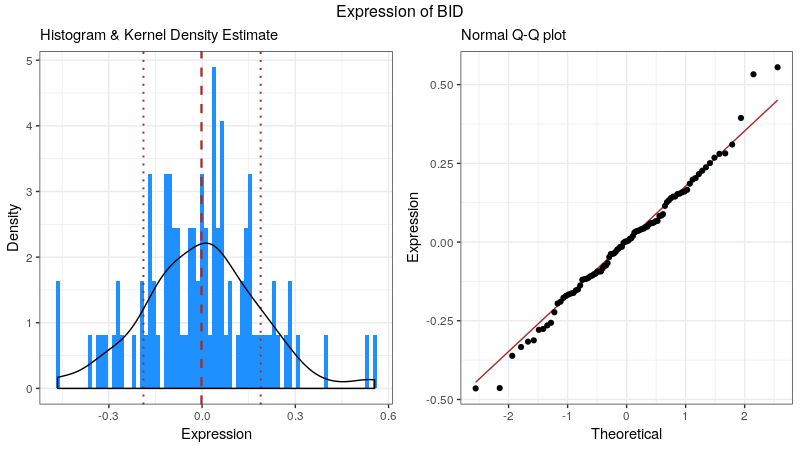
\includegraphics[height=4.8cm,width=.8\textwidth,keepaspectratio=false]{bid_expr}
  \end{subfigure}
%\end{figure}

  \begin{subfigure}{\textwidth}
%\begin{figure}[t]
    \centering
    \caption{}
% 	\caption{Scree plot and biplot of 
% the \textasciitilde800 affinities for the gene BID. In the biplot, each 
% label corresponds to an individual.}
    \labfig{pcatba}
    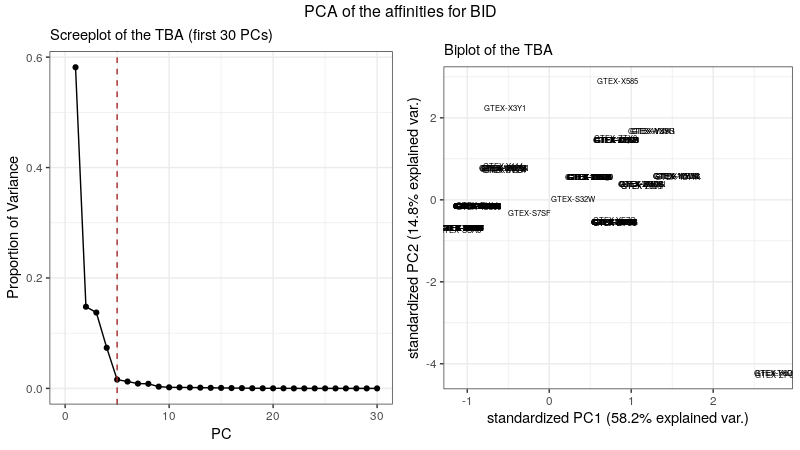
\includegraphics[height=4.8cm,width=.8\textwidth,keepaspectratio=false]{bid_tba}
  \end{subfigure}
% \end{figure}
  \caption{(a): Histogram and normal Q\babelhyphen{nobreak}Q plot of the 
expression of a randomly selected gene called BID. In the histogram, the 
brown dashed line indicates the mean, while the dotted lines indicate 
plus and minus one standard deviation. In the Q\babelhyphen{nobreak}Q 
plot, each point represents an individual. (b): Scree plot and biplot of 
the \textasciitilde800 affinities for the gene BID. In the biplot, each 
label corresponds to an individual.}
  \labfig{expl}
\end{figure}

The expression was preprocessed as recommended by the Stephen's 
Lab.\sidenote[][*7]{\url{http://stephenslab.github.io/gtex-eqtls/analysis/20170515\_RNASeq\_Analysis.html}} 
In summary, I applied a quantile normalisation to make sure that the 
distribution of our response variable was normal, and then I obtained 
the residuals of a linear model 
$Y~\sim~SEX+PEER\_FA+POPULATION+PLATFORM$, so as to disregard the 
effects of these covariates on the expression. The final result can be 
seen in \reffig{distrexpr}.

The genotypes were also obtained with a sequencing technique and were 
provided in VCF format. \sidecite[-3.2cm]{Danecek2011} I 
used a software called 
\nohyphens{VCF\textunderscore\nobreak\hspace{0pt}rider}\sidenote[][*3]{\url{https://github.com/vodkatad/vcf\_rider}} 
to compute the total binding affinity of each transcription factor for 
each regulatory region associated to a gene (the total number of 
transcription factors is about 800). \reffig{pcatba} reports the PCA of 
the TBA for the gene BID.

\section{Results}
\labsec{results}

\subsection{Nested Cross-Validation Package}

All the similar published works use a 5-fold cross-validation to 
evaluate their models. However, since there are also some parameters to 
tune, they rely on a (computationally expensive) netsed cross-validation 
in order not to overestimate the predictive power. Since I needed to run 
several different models for each of the 140 genes, each with its own 
parameters, I decided to write an R 
package\sidenote[][-2.3cm]{\url{https://github.com/fmarotta/cvtools}} to 
perform the nested cross-validation with a heuristic algorithm that does 
not try all the possible values for the parameters, but rather, 
independently for each parameter, it starts at one value and explores 
the adjacent ones; then, it moves in the direction where the error 
decreases
(\reffig{cv}).

\begin{marginfigure}[-3.4cm]
  \centering
  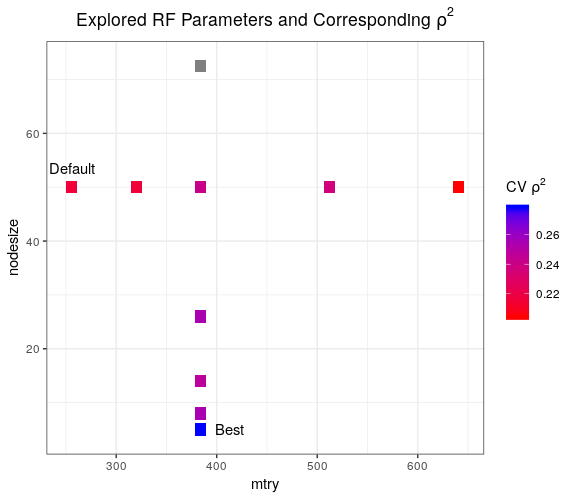
\includegraphics{cv}
  \caption{First, the mtry is tuned while the nodesize is kept fixed; 
the algorithm started at the default value of 256, then it moved up in 
the range as long as the error decreased, and finally it came back to 
explore the values in between. Next, the nodesize was tuned in a similar 
fashion.}
  \labfig{cv}
\end{marginfigure}

This package requires the user to write a function which takes 
predefined arguments and returns a predefined output, but except for 
that, it can be used with any regression model. I evaluated the 
performances of ridge, BART, random forest, and PCR. 
\sidecite[-12.9cm]{James2013a,Hastie2009}

\subsection{Model Performance}

The measure of performance is not the MSE nor the $R^2$, but rather the 
square of the correlation between true and predicted expression 
($\rho^2$); indeed, we do not want to penalise errors on single 
individuals, but we are interested in the general trend of expression. I 
decided to compare my results with those of TIGAR, \cite{Nagpal2019} 
which is currently most recent paper on this topic.

\begin{table}[b]
  \caption{Mean $\rho^2$ across 141 genes. The t-test was always 
performed with respect to TIGAR.}
  \labtab{comp}
  \begin{tabular}{lcc}
  \textbf{Model} & \textbf{Mean} \boldmath$\rho^2$ & \textbf{t-test pval} \\
  \midrule
  TIGAR & 0.067 & NA\\
  Ridge & 0.076 & 0.025\\
  BART & 0.074 & 0.121\\
  Ranger & 0.069 & 0.398\\
  PCR & 0.064 & 0.737\\
  \end{tabular}
\end{table}

Even if it captures only the linear relationships, ridge gave the best 
predictive performance (\reffig{rho2distr}), probably because in this 
context where $p >> n$, it is a good compromise between bias, variance 
and overfitting. According to a t-test, the $\rho^2$ achieved by ridge 
with the TBA values are even higher than those obtained by TIGAR 
(\reftab{comp}).

\begin{marginfigure}[-2cm]
  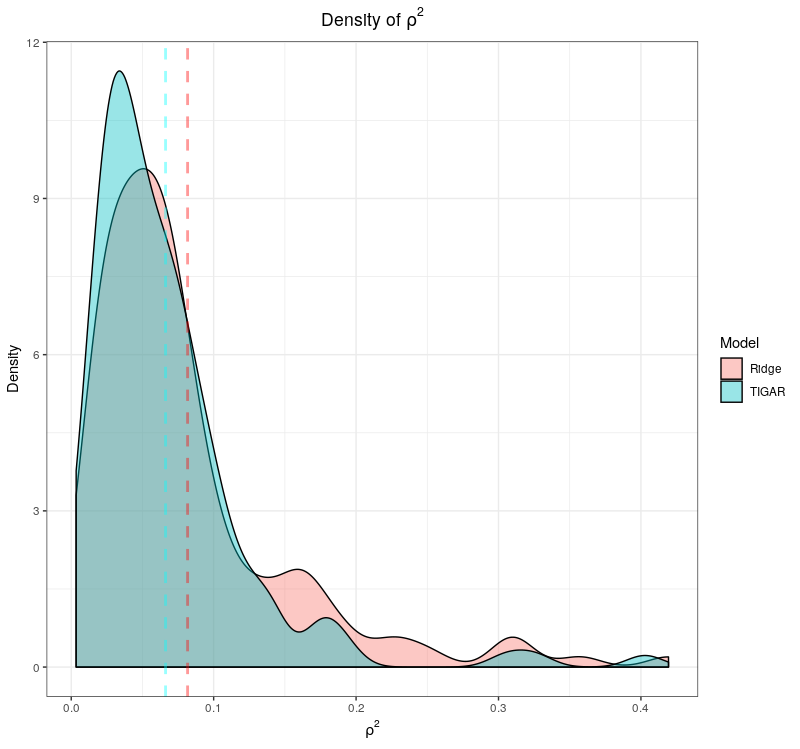
\includegraphics{rho2distr}
  \caption{Density plot of the $\rho^2$ achieved by T-REx (Ridge) and 
TIGAR. The dotted lines denotes the means of the 
distributions.}
  \labfig{rho2distr}
\end{marginfigure}

The performance of BART was not so different, despite the method being 
completely different. However, an important advantage of BART with 
respect to ridge is its ability to provide importance measures, allowing 
us to find which transcription factors are important for each gene. 
Additionally, BART captures the interactions between transcription 
factors.

The other methods, random forest and principal component regression, 
were much less powerful.

\subsection{Considering the Expression of the Transcription Factor}

As high as its affinity for the DNA may be, if the transcription factor 
is present only in tiny amounts it will not bind many regulatory 
regions. For this reason, we tried to enhance our predictors with 
information from the expression of the transcription factors.

\marginnote{%
The Hill equation models the rate of expression of a gene:
\begin{equation*}
  \theta = w \frac{L^n}{K^n + L^n} \approx w \left(\frac{L}{K}\right)^n.
\end{equation*}
Here, $L$ is the amount of transcription factor, $K$ is the dissociation 
constant (the inverse of the affinity), and $w$ is a constant. It is 
reasonable to suppose that if many transcription factors regulate a 
gene, the rate will be given by the following product, where we denoted 
$A = 1 / K$:
\begin{equation*}
  \theta = w_1 \left( L_1 A_1 \right)^{n_1} \cdots w_p \left( L_p A_p \right)^{n_p}.
\end{equation*}
Now, if we compute the log of the rate, we get a linear combination 
which in principle is a deterministic function, but in practice we can 
use this linear combination as the right-hand side of a model formula 
and let ridge estimate the coefficients:
\begin{align*}
  Y \sim \beta_0 &+ \beta_1 \left(\log L_1 + \log A_1\right) \\
                 &+ \cdots \\
                 &+ \beta_p \left(\log L_p + \log A_p\right).
\end{align*}
}

In the dataset, we have expression values for some 40.000 genes; of 
these, about 800 are transcriptional factors. In practice we removed 
those rows from the dataset, and summed the TBA and the expression of 
corresponding transcription factors. The new predictors gave a 
considerable improvement in the performance, and, perhaps surprisingly,
ridge outclassed BART. In the adjacent margin note I describe the 
working hypothesis more in detail.

\begin{table}[H]
  \begin{tabular}{lr}
  \textbf{Model} & \textbf{Mean} \boldmath$\rho^2$ \\
  \midrule
  Ridge & 0.393\\
  BART & 0.268\\
  \end{tabular}
\end{table}


\section{Discussion}
\labsec{discussion}

Instead of finding a better model, in this project I tried to find 
better predictors. Using the affinities instead of the genotypes has 
several advantages:

\begin{itemize}
  \item The model is more interpretable;
  \item The number of predictors decreases;
  \item The predictive power is higher;
\end{itemize}

Upon doing some biochemical considerations, it is possible to find even 
better predictors, although they violate the constraint of using only 
the DNA sequence to predict gene expression.

There are many ways to continue this work. One would be to construct an 
ensemble model that chooses, for each gene, the model that achieved the 
best prediction on a training set.

Another possibility is that of exploiting further the interpretability 
of this model, and use the trees produced by BART to make inferences 
about the regulatory network among genes.

Finally, one of the biggest limitations of these kind of models is that 
they consider each gene as independent of all the others. One possible 
way to use the information hidden among other genes is what I call the 
\enquote{bagging of the genes,} where the prediction for a new gene is 
given by the average of the prediction of a number of other models 
trained on different genes.

If we were able to accurately predict gene expression, the benefit would 
be twofold: first, it would be possible to predict which individuals are 
at risk of developing a disease, and consequently to prevent it; 
secondly, the biological mechanisms through which the illnesses arise 
would be elucidated, potentially leading to the discovery of new 
therapeutic targets. In conclusion, I hope that this project will give a 
contribution, albeit very small, in understanding the relationships 
between genome, expression and diseases.


\defbibnote{bibnote}{Here are the references in citation order.\par\bigskip} % Prepend this text to the bibliography
\renewcommand*{\bibfont}{\small}
\printbibliography[title=Bibliography]% , prenote=bibnote]

\end{document}
